\documentclass[xcolor=dvipsnames, aspectratio = 169]{beamer}
\usepackage[english]{babel} %% english
\usepackage[utf8]{inputenc}
\usepackage[T1]{fontenc}
\usepackage{include/chariteBeamer}
\usepackage{hyperref}
\author[E. Sprünken]{Erin Sprünken}
\institute[]{
Institut für Biometrie und Klinische Epidemiologie\\[1Ex] 
Charité - Universitätsmedizin Berlin, Berlin\\[1Ex]
erin-dirk.spruenken@charite.de} 
\titlegraphic{\pgfuseimage{frontUnilogo}}

\tikzset{>=latex}
%\usepackage{amsmath}
%\usetikzlibrary{shadows}
\usepackage[edges]{forest}
\usetikzlibrary{positioning}
\usepackage{biostat}
\setbeamertemplate{caption}[numbered]
\let\qed\relax
\forestset{declare toks={elo}{}}
\graphicspath{{figures/}}
%% ================================================================== %% 

\author[L. Mödl, M. Becher, E. Sprünken]{Lukas Mödl, Matthias Becher, Erin Sprünken} 
\title{R-Course: Day 1} 
\date[]{\today}

%% ================================================================== %% 
\setbeamercolor*{mycol}{bg=chariteGray, fg=chariteBlue}

\hyphenation{Sam-ples}
\begin{document}

%% ================================================================== %%
%% ================================================================== %%
\setbeamertemplate{footline}{\begin{tikzpicture}
    \node [inner sep=0pt, anchor=east] (0,0) {
      
\includegraphics[width=\paperwidth,height=0.7cm]{include/charite_footer}};
    \node [inner sep=0pt, anchor=east] at (-0.5ex,-0ex){};
\end{tikzpicture}}

\setbeamertemplate{headline}{
%\leavevmode
\hspace{-0.49em}\hbox{
	\begin{beamercolorbox}[wd=1.02\paperwidth,ht=2.25ex,dp=1ex,left]{mycol}%
    \usebeamerfont{section in head/foot}
  \end{beamercolorbox}%
}}
{
  \usebackgroundtemplate{ \hspace{-0.5em}\begin{tikzpicture}
  \node[opacity=0.7, anchor=south] (0,0) {
\includegraphics[height=\paperheight, width=1.04\paperwidth]{include/frontmatter.pdf}};
  \end{tikzpicture}
} 
%\frame{\titlepage}
\begin{frame}
\centering
	\vspace{4em}
	{\Large \textcolor{chariteBlue}{\inserttitle}}\\
	 \vspace{1em}
	{\Large \textcolor{black}{\insertauthor \\}} 
	\vspace{2em}
	{\footnotesize \textcolor{black}{\insertinstitute \\\vspace{1em} \insertdate}} 
	\vspace{0em}
	\begin{figure}[h!]
		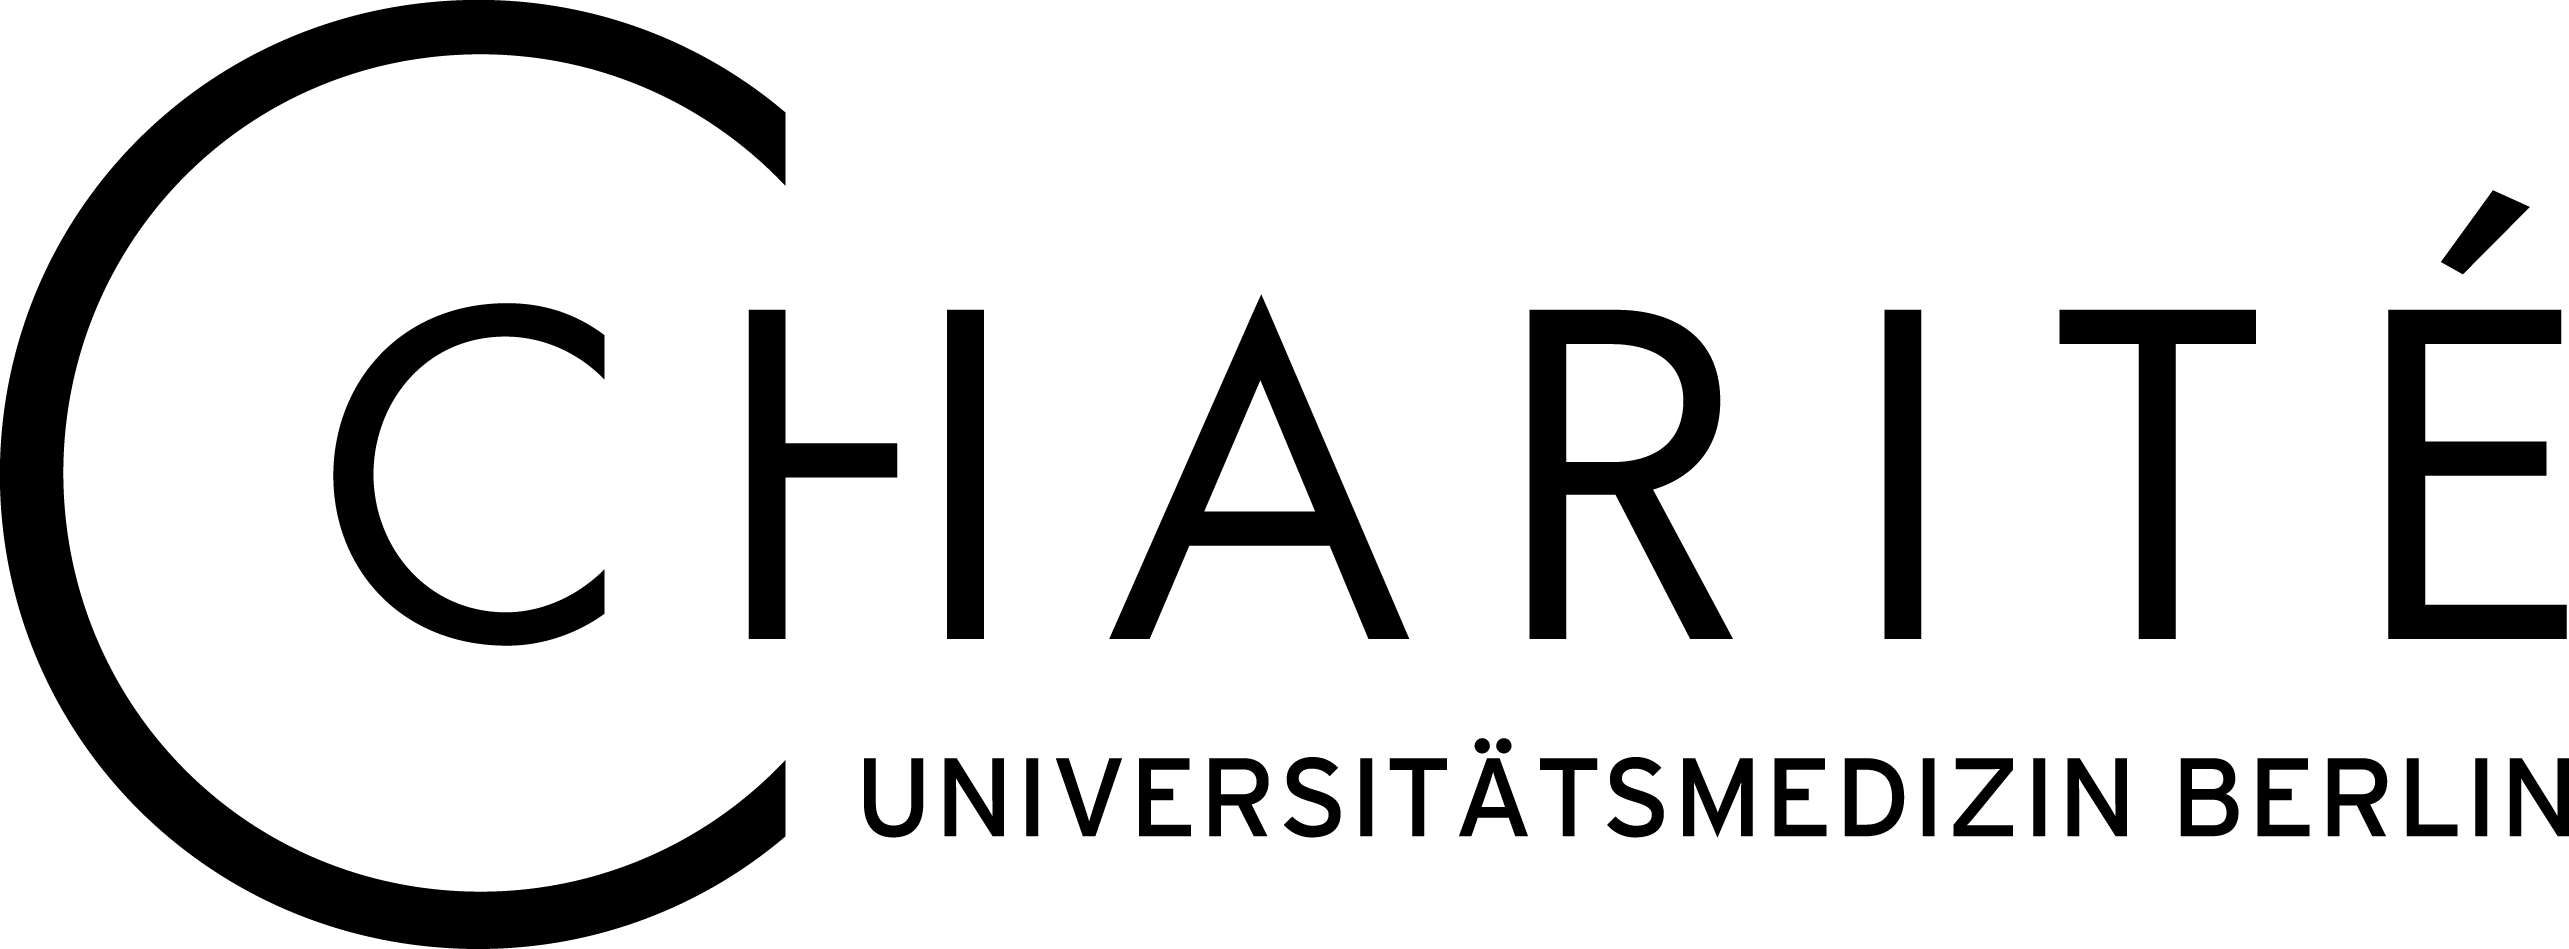
\includegraphics[width=5cm]{include/Charite_Logo.png}
	\end{figure}
%	\pgfuseimage{frontUnilogo}
\end{frame}
}
%% ================================================================== %%

\setbeamertemplate{footline}{\begin{tikzpicture}
    \node [inner sep=0pt, anchor=east] (0,0) {
      
\includegraphics[width=\paperwidth,height=0.7cm]{include/charite_footer}};
    \node [inner sep=0pt, anchor=east] at (-0.5ex,-0ex) {\tiny \insertframenumber{}$\,$|$\,$\inserttotalframenumber};
\end{tikzpicture}}

\setbeamertemplate{headline}{%
%\leavevmode%
\hspace{-0.49em}\hbox{
	\begin{beamercolorbox}[wd=.68\paperwidth,ht=2.25ex,dp=1ex,left]{mycol}%
    \usebeamerfont{section in head/foot}\hspace*{1em}
  \end{beamercolorbox}%
  \begin{beamercolorbox}[wd=.20\paperwidth,ht=2.25ex,dp=1ex,right]{mycol}%
    \usebeamerfont{author in head/foot}\insertshortauthor
  \end{beamercolorbox}%
  \begin{beamercolorbox}[wd=.14\paperwidth,ht=2.25ex,dp=1ex,center]{mycol}%
    \usebeamerfont{date in head/foot}\insertdate
  \end{beamercolorbox}%
  }
}


\frame{\tableofcontents}

\setbeamertemplate{headline}{%
%\leavevmode%
\hspace{-0.49em}\hbox{
	\begin{beamercolorbox}[wd=.68\paperwidth,ht=2.25ex,dp=1ex,left]{mycol}%
    \usebeamerfont{section in head/foot}\hspace*{1em}\thesection. \  \insertsectionhead
  \end{beamercolorbox}%
  \begin{beamercolorbox}[wd=.20\paperwidth,ht=2.25ex,dp=1ex,right]{mycol}%
    \usebeamerfont{author in head/foot}\insertshortauthor
  \end{beamercolorbox}%
  \begin{beamercolorbox}[wd=.14\paperwidth,ht=2.25ex,dp=1ex,center]{mycol}%
    \usebeamerfont{date in head/foot}\insertdate
  \end{beamercolorbox}%
  }
}

\section{Introduction}
\begin{frame}[fragile]{Motivation}
  \begin{itemize}
  \item Statistical Analyses
  \item Possibilities compared to SPSS, SAS, Stata
  \item Open Source
  \end{itemize}
\end{frame}


\begin{frame}{Installation}
	\begin{itemize}
		\item \href{https://www.r-project.org/}{R (Software)  
\includegraphics[scale=0.01]{include/r-logo}}
		\item \href{https://www.rstudio.com/}{RStudio (GUI = Graphical User Interface)  
\includegraphics[scale=0.04]{include/rstudio-logo}}
		\item Alternatives (but not recommended by us): xcode, Visual Studio, Texteditor
	\end{itemize}
	
\end{frame}

%% ================================================================== %%
\section{How to communicate with R?}

\begin{frame}{Interface of RStudio}
\begin{columns}[T]
	\begin{column}{0.6\textwidth}
	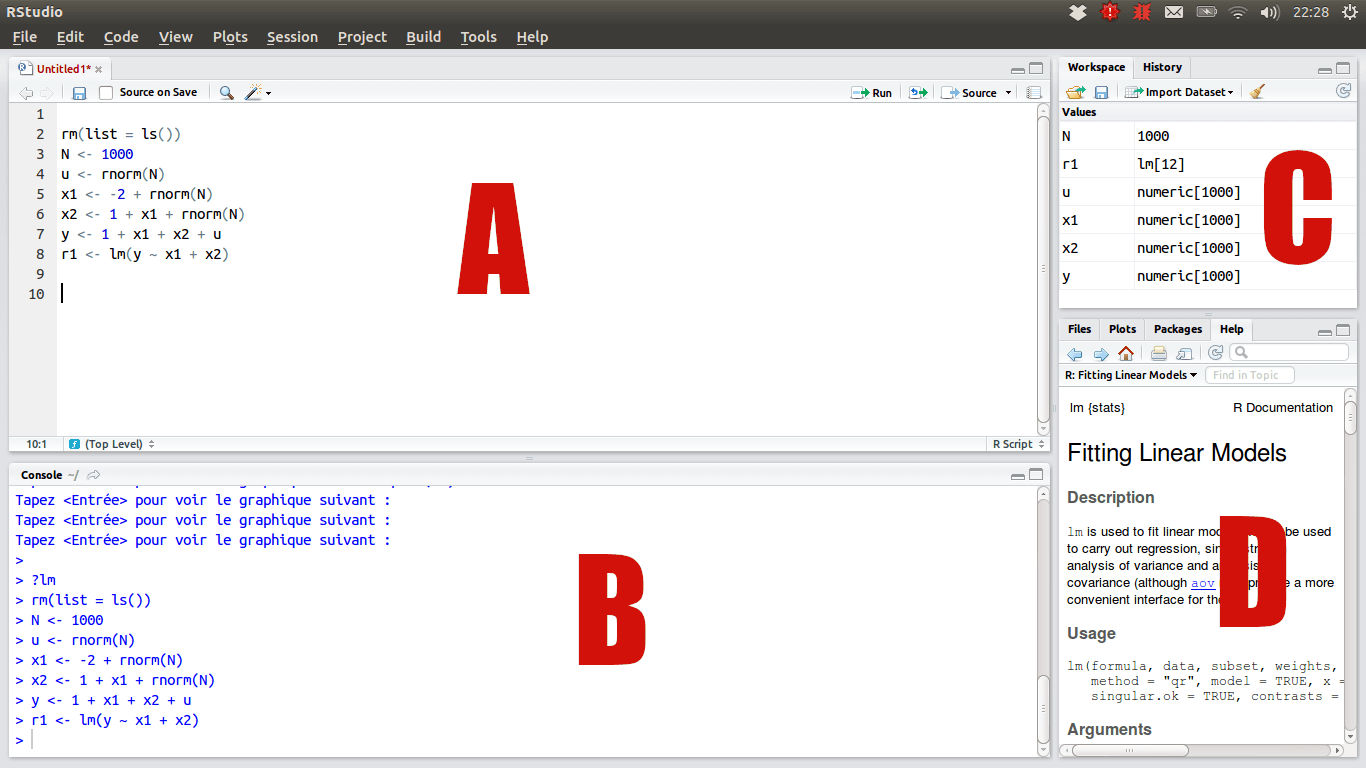
\includegraphics[scale=0.65]{Rstudio_interface1}
	\end{column}
	\begin{column}{0.4\textwidth}
	\begin{enumerate}
		\item[A] Script window
		\item[B] Console
		\item[C] Workspace, Data
		\item[D] Plots, Help, Filebrowser, Packet manager
	\end{enumerate}
	\end{column}
\end{columns}
\end{frame}
\begin{frame}{Console and Pocket Calculator}
	\begin{columns}[T]
	\begin{column}{0.6\textwidth}
	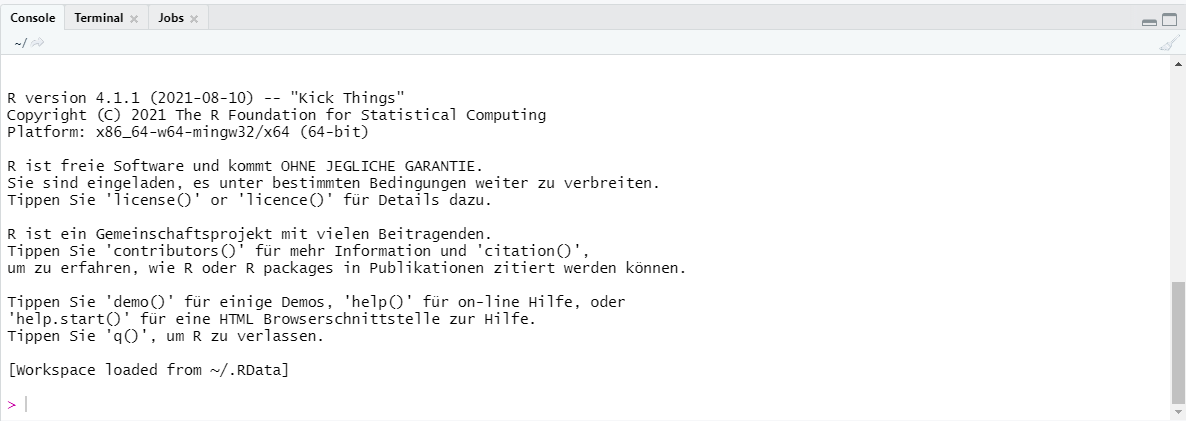
\includegraphics[width=\textwidth]{Rstudio_interface_c}
	\end{column}
	\begin{column}{0.4\textwidth}
	\begin{itemize}
		\item Only \glqq Console\grqq{} relevant
		\item We can write commands and execute them with enter
		\item Example pocket calculator:
		\begin{itemize}
			\item 3 + 2
			\item 5 * 4
			\item 20 - 8
			\item 12 / 16
		\end{itemize}
	\end{itemize}
	\end{column}
\end{columns}
\end{frame}

\begin{frame}[fragile]{Errors, Warnings, NA, NaN, Inf}
	What happens if we write \verb+ 5!+ ? \\
	R gives us an error. It is important that we know what to tell R. Thus: \verb+ factorial(5)+. \\
	\begin{itemize}
		\item 3 / 0 $\Rightarrow$ \verb+ Inf+; R solves this numerically and ends up with a limit (here \verb+ Inf+ $=\infty$).
		\item 0/0 $\Rightarrow$ \verb+ NaN+; stands for \glqq Not a Number\grqq{}
		\item NA stands for "Not Available", i.e. a missing value. The main reason for this to occur (aside from raw data) is, if we conduct operations and don't tell R how to handle missing data.
	\end{itemize}

\end{frame}

\begin{frame}[fragile]{Mathematical Expressions}
	\begin{itemize}
		\item \verb+ factorial(x)+ $= x!$
		\item \verb+ exp(x)+ $=e^x$
		\item \verb+ log(x)+ $=log(x)$
		\item \verb+ sqrt(x)+ $=\sqrt{x}$
		\item \verb+ abs(x)+ $=\abs{x}$
		\item \verb+ x^n + $=x^n$
	\end{itemize}
\end{frame}

\begin{frame}{Script window}
	\begin{columns}[T]
	\begin{column}{0.6\textwidth}
	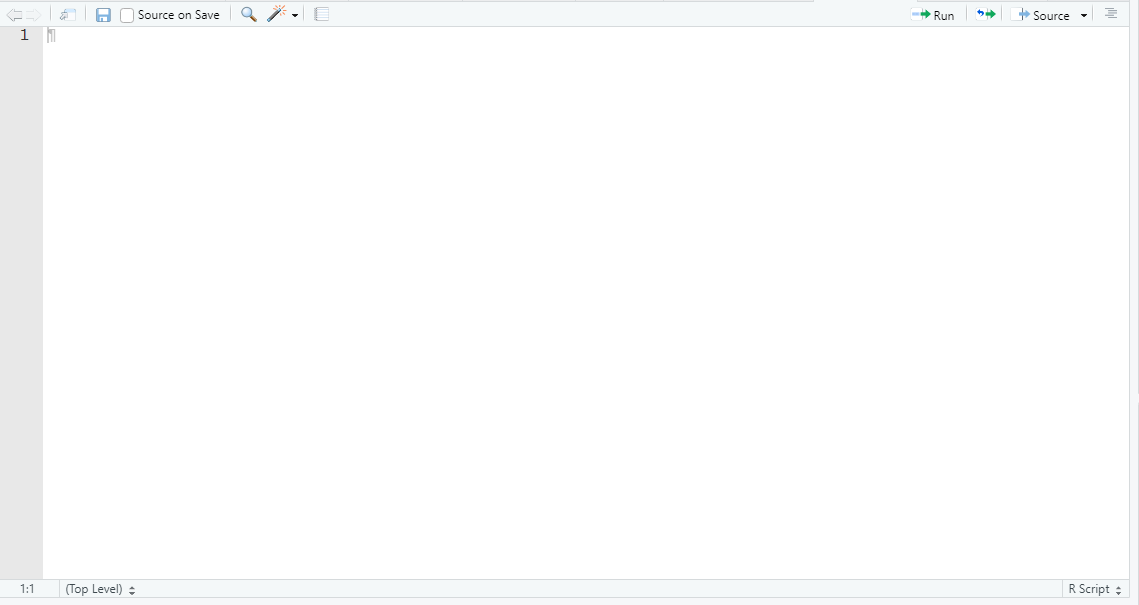
\includegraphics[width=\textwidth]{Rstudio_interface_i}
	\end{column}
	\begin{column}{0.4\textwidth}
	\begin{itemize}
		\item \small It is inconvenient to write every command line by line into the console
		\item \small Here, we can write as many commands as we want after another and execute whole blocks
		\item \small On the technical side, R just hands over the executed lines from the script to the console line by line
		\item \small Scripts can be saved and reused
	\end{itemize}
	\end{column}
\end{columns}
\end{frame}

\begin{frame}[fragile]{Assigning variables}
Often, we want to save results or data for later use. To do so, we must assign variables. Historically, the left-pointing arrow is used in R: \verb+<-+. The common \verb+=+ works just as well. Variables are case-sensitive!
\begin{itemize}
	\item \verb+ x <- 3.1415+
	\item \verb+ b <- 4+
	\item \verb+ B = 5+
	\item \verb+ d <- factorial(5)+
\end{itemize}
\end{frame}

\begin{frame}[fragile]{Other}
R offers several usefule functions. Two specifically useful are \verb+?+ and \verb+rm()+
\begin{itemize}
	\item If we want to know how a functions works, we can type the question mark followed by the name of the function to call the documentation, e.g.: \verb+?rm+
	\item If we do so, we get the information about \verb+rm()+: We can write objects into the parentheses that we want to remove. From the former slide we have \verb+x+, \verb+b+, \verb+B+ and \verb+d+
	\item We want to remove \verb+B+ and \verb+b+, thus: \verb+ rm(B, b)+
\end{itemize}
\end{frame}

%% ================================================================== %%
\section{Daten}
\begin{frame}[fragile]{Datatypes}
	What types of data exist in R?
	\begin{itemize}
		\item Numeric $\Leftrightarrow$ Numbers, \verb+is.numeric()+
		\item Character $\Leftrightarrow$ Letters/Words, \verb+is.character()+
		\item Factor $\Leftrightarrow$ Categorical Variables, \verb+is.factor()+
		\item Date $\Leftrightarrow$ Date/Time
		\item Logical $\Leftrightarrow$ True/False, \verb+is.logical()+
	\end{itemize}
\end{frame}

\begin{frame}[fragile]{Vector}
	R is a vector-language: Most of the data constructions are types or expansions of a vector.\\
	A vector in R can only contain a single datatype.
	\begin{itemize}
		\item \verb+ c()+
		\item \verb+ seq()+
		\item \verb+ rep()+
		\item \verb+ is.vector()+
	\end{itemize}
\end{frame}

\begin{frame}[fragile]{Matrix}
	A matrix is a chaining of vectors (side-by-side, row-by-row).\\
	A matrix in R can only contain a single datatype.
	\begin{itemize}
		\item \verb+ matrix()+
		\item \verb+ cbind()+
		\item \verb+ rbind()+
		\item \verb+ is.matrix()+
	\end{itemize}
\end{frame}

\begin{frame}[fragile]{Algebraic operations}
It is simple to calculate with vectors and matrices in R. By default, R computes everything elementwise. What do we get using the following command?\\
\verb+ c(3.1415, 5, 1, 2/3) * seq(1, 8, 2)+ \\
R computes as follows: \begin{align*}
	\begin{pmatrix}
	3.1415 \\ 5 \\ 1 \\ \frac{2}{3}
	\end{pmatrix} \quad * 
	\underbrace{\begin{pmatrix}
		1 \\ 3 \\ 5 \\ 7
	\end{pmatrix}}_{\text{seq(1, 8, 2) = c(1, 3, 5, 7)}}
	\quad &= \quad \begin{pmatrix}
	3.1415 \cdot 1 \\
	5 \cdot 3 \\
	1 \cdot 5 \\
	\frac{2}{3} \cdot 7
	\end{pmatrix}
\end{align*}
\end{frame}

\begin{frame}[fragile]{List}
	Maybe we want to store different datatypes in a vector, what can we do now?\\
	Answer: List.\\
	Lists are generalized forms of the classical vector, as elements of a list are not restricted to the same datatype. Lists are extremely flexible and can be nested into each other, i.e. a list can contain lists.
	\begin{itemize}
		\item \verb+ list()+
		\item \verb+ c()+
		\item \verb+ $ +
	\end{itemize}
\end{frame}

\begin{frame}[fragile]{Data Frame}
	However, lists can become confusing. A special type of a list is the Data Frame.
	Visually, it looks just like a matrix, but the Data Frame is allowed to store different datatypes in different columns. However, a single column must contain data from only one datatype.
	\begin{itemize}
		\item \verb+ data.frame()+
		\item \verb+ rbind()+
		\item \verb+ cbind()+
		\item \verb+ $+
	\end{itemize}
\end{frame}

\section{Saving Data}

\begin{frame}[fragile]{Saving}
	Typically, we don't work on something only once. For this it seems useful that we save data. R offers a file format to save data for later use: \verb+*.RData+
	\begin{itemize}
		\item \verb+ save()+
		\item \verb+ write.table()+
		\item \verb+ write.csv()+
	\end{itemize}
\end{frame}

\end{document}
%% ================================================================== %%
%% ================================================================== %% 
